% ============================================================
% QM-1: Emergence of the Schrödinger Equation from Sea-Polarization
%       Pattern Dynamics (formerly: from DI-Bit Hopping)
% Version 2.0 — 4 August 2026
%
% CHANGELOG:
%   v1   Mar 2026  — Initial draft
%   v1.1 2 Apr 2026 — Formatting compliance: .bib, natbib,
%                     graphicspath, TOC, PLS, OSF DOI
%   v2.0 4 Aug 2026 — PATTERN-LEVEL RE-GROUNDING (OPEN-QM-1-REGROUND,
%                     Patches 2988/2995/2996/2997). The per-bit
%                     phase-accumulation grounding is RETIRED under
%                     founder ruling 2957 P-1 + A1' reset-per-hop
%                     (audit: series_quantum_mechanics/
%                     qm1_phase_provenance_audit.md). The site field
%                     is re-grounded on FI-QMRG-1 (phi = orientation
%                     of the GP's SSV_net directional content in the
%                     distinguished ZBW plane; rho = the count-like
%                     SSV_abs register). Eq. (phasehop) replaced by
%                     the pattern-rotation equation (same numerical
%                     content, corrected bearer). Unitarity grounded
%                     in reversible conserved PCD displacement.
%                     Theorem statement and proof UNCHANGED (the 2988
%                     audit's Finding S-1: the mathematics never
%                     consumed per-bit phase). Anti-erasure notes
%                     throughout. Title-block version marker
%                     reconciled with this CHANGELOG (pre-2.0 title
%                     carried a stale "(Version 3.1)").
%   v2.1 4 Aug 2026 — CONV-014 PANEL AMENDMENTS ENACTED (adjudication
%                     Patch 3000, 4-1 on Q1): (a) A-1 restated as
%                     natural-availability, not uniqueness
%                     (OPEN-QMRG-UNIQ registered); (b) FI-QMRG-1 now
%                     carries two explicit conditions — C-i the
%                     amplitude-count magnitude constraint (B-QMRG-1)
%                     and C-ii plane stability under GP refresh (R-4,
%                     severity medium-high); (c) node-singularity
%                     wording downgraded to consistency-by-
%                     construction; (d) OPEN-QMRG-B1 mandatory-
%                     derivation + mutual-support prohibition noted
%                     in the Grade remark. Mathematics unchanged.
%   v2.2 4 Aug 2026 — R-4 STATUS UPDATE (Patch 3001): plane stability
%                     advanced to CLOSURE CANDIDATE at derivation
%                     grade, panel-pending — the 5-design lemma
%                     package (exact closure for the shipped
%                     component-diagonal transport; (k Delta-s)^4
%                     suppression of the lattice-anisotropic channel
%                     from the icosahedral spherical-5-design theorem,
%                     numerically verified with negative control;
%                     the isotropic direction-coupled channel
%                     identified as the spin/longitudinal sector).
%                     Record: sketches/3001_r4_plane_stability_lemma.md
%                     + code/3001_r4_5design_check.py (ALL PASS).
%                     Grade remark updated; mathematics unchanged.
%   v2.4 4 Aug 2026 — CONV-015 ADJUDICATION ENACTED (Patch 3004):
%                     R-4 CLOSED at derivation grade for the shipped
%                     transport class (Q1 5-0; residue spun off as
%                     OPEN-QMRG-R4-MULTILINK); OPEN-QMRG-B1 CLOSED at
%                     proportionality grade (Q2 5-0; dependency order
%                     amended — the energy balance is load-bearing,
%                     AP-2 is register identification; exact
%                     coefficient -> OPEN-QMRG-B1-CONST); the
%                     QM-1<->QM-5 mutual-support prohibition
%                     DISCHARGED with the citation rider; conditional-
%                     note obligations now MULTILINK + B1-CONST.
%                     Grade remark updated; mathematics unchanged.
%   v2.5 4 Aug 2026 — OPEN-QMRG-R4-MULTILINK STATUS UPDATE (Patch
%                     3005): advanced to RESOLUTION CANDIDATE at
%                     registry-theorem grade, panel-pending — the
%                     committed refresh law FORCES the single-edge
%                     kernel class by three ratified clauses (A3'
%                     additive vector-sum register formation; AP-2
%                     minimal messenger content; A3' per-Moment
%                     reset); the committed chirality mechanism (F.1
%                     Mechanism A, per-edge scalar rate asymmetry) is
%                     Channel A and plane-exact under any weights;
%                     quantitative moat verified (symmetric cross-
%                     sums vanish; separable pair kernels exact or
%                     slope-4; the EXCLUDED non-separable chiral
%                     class leaks at ORDER UNITY — the exclusion is
%                     maximally load-bearing). Watch condition
%                     W-MULTILINK-1 registered. Record: sketches/
%                     3005_multilink_refresh_law_analysis.md + code/
%                     3005_multilink_pair_kernel_check.py (ALL PASS).
%                     Grade remark updated; mathematics unchanged.
%   v2.6 4 Aug 2026 — OPEN-QMRG-B1-CONST STATUS UPDATE (Patch 3006):
%                     advanced to DISPOSITION CANDIDATE (derive-and-
%                     quarantine), panel-pending. LAYER 1 DERIVED:
%                     in the declared convention (cycle-averaged
%                     mean-square in-plane register), the virial
%                     coefficient is EXACTLY 1 — <S_perp^2> =
%                     N hbar/(mu omega) given E = N hbar omega — and
%                     the canonical per-quadrature 1/2 is DERIVED as
%                     the two-quadrature split of the rotating ZBW
%                     pattern (verified to 6 decimals). LAYER 2
%                     QUARANTINED: eta = rho/N (count-to-occupation
%                     participation ratio), the ONE lattice-dependent
%                     unknown, registered with a checkable mode-
%                     independence claim; separation verified — the
%                     coefficient is invariant across a x17 turnover
%                     scan. Record: sketches/
%                     3006_b1const_convention_derivation.md + code/
%                     3006_b1const_coefficient_check.py (ALL PASS).
%                     Both trigger items now candidates: CONV-016
%                     ready. Grade remark updated; math unchanged.
%   v2.7 4 Aug 2026 — TERMINAL STATUS (CONV-016 adjudication, Patch
%                     3008): the QM sector's CONDITIONAL status
%                     (imposed Patch 2988) is RESOLVED (Q3 3-2 per
%                     the pre-registered E-6 mapping; Q1 5-0, Q2 5-0,
%                     Q5 4-1); the citation bar is WIDENED NEAR-FULL
%                     (Q4 2-2-1: full lift failed only its majority
%                     conjunct; scope authority conv016_adjudication
%                     sec.6 E-2); MULTILINK RESOLVED (scope: the
%                     presently ratified refresh construction);
%                     B1-CONST DISPOSED (E=N hbar omega provenance
%                     audited ACYCLIC: SF-6 Tier-1, shipped pre-arc,
%                     c06 basis; eta consumption sweep clean).
%                     Persisting ORDINARY items: OPEN-QMRG-ETA,
%                     OPEN-QMRG-UNIQ, W-MULTILINK-1. Grade remark
%                     final form; mathematics unchanged since v1.1.
%   v2.8 4 Aug 2026 — OPEN-QMRG-ETA STATUS (Patch 3009, ordinary
%                     bookkeeping): eta's MODE-INDEPENDENCE DERIVED
%                     at lattice-bookkeeping grade — a cancellation
%                     between the A3' universal Moment-cadence
%                     turnover (content/Moment ~ N hbar omega) and
%                     the I-3 quantum-per-transit scaling (hbar
%                     omega per messenger): the omegas cancel,
%                     eta = c_geo, a pure relay-geometry constant.
%                     Both ingredients shown individually load-
%                     bearing by negative controls. Item remains
%                     open at reduced scope (the value c_geo only);
%                     the eta-universality note class becomes
%                     dischargeable at the next panel touchpoint.
%                     Record: sketches/3009_eta_lattice_derivation.md
%                     + code/3009_eta_mode_independence_check.py
%                     (ALL PASS). Mathematics unchanged.
%   v2.12 10 Aug 2026 — AUX-2 DISCHARGE (CONV-017, 5/5 riding
%                     AUX-1 CLOSE; Patch 3050): eta-universality
%                     note class discharged; persisting notes now
%                     uniqueness + universal-microscopic (the final
%                     two). Mathematics untouched.
%   v2.11 9 Aug 2026 — AUX-3 DISCHARGE RECORDED (Patch 3037,
%                     CONV-013 3/5): the physical rho-calibrated-
%                     normalization note class discharged at
%                     bookkeeping grade; note-class list and the
%                     barred sentence amended with the grade fence;
%                     eta-universality/uniqueness/universal-
%                     microscopic notes persist. Mathematics
%                     untouched.
%   v2.10 8 Aug 2026 — O-7 SWEEP (Patch 3033, AP-4 ratified 3032):
%                     DI-bit content citations updated to {origin
%                     address, E, S}; no-phase/count-like preserved;
%                     3005/3002 premises flagged under O-6/W-MULTILINK-1
%                     (re-derivation BLOCKING for AP-4-dependent
%                     shipping). Mathematics untouched.
%   v2.9 4 Aug 2026 — OPEN-QMRG-ETA COMPLETION (Patch 3010): the
%                     value computed — c_geo = z = 12 (Version B
%                     relay, standing class, interior sites);
%                     class-dependent / mode-independent-within-
%                     class refinement stated; INERTNESS VERIFIED
%                     (virial coefficient and physical ratios
%                     convention-blind). Item -> CLOSURE CANDIDATE,
%                     batched for the next panel touchpoint.
%                     Record: sketches/3010_cgeo_relay_bookkeeping.md
%                     + code/3010_cgeo_relay_multiplicity_check.py
%                     (ALL PASS). Mathematics unchanged.
%   v2.3 4 Aug 2026 — OPEN-QMRG-B1 STATUS UPDATE (Patch 3002): the
%                     amplitude-count bridge advanced to DERIVATION
%                     CANDIDATE at derivation grade, panel-pending —
%                     derived from elastic energy balance (SF-6 Sea
%                     stiffness + A3' per-Moment turnover + the
%                     hbar-omega energy quantum per messenger), with
%                     the quadratic-vs-linear fork resolved by
%                     ratified AP-2's intensity-like clause and the
%                     canonical 1/(2 omega) normalization RECOVERED
%                     as an output (anti-circularity: QM-5 quantization
%                     consumed nowhere). Verified with negative
%                     control. Record: sketches/
%                     3002_b1_amplitude_count_derivation.md + code/
%                     3002_b1_energy_balance_check.py (ALL PASS).
%                     Grade remark updated; mathematics unchanged.
%
% FIGURE PATH:
%   .tex: series_quantum_mechanics/papers/
%   figs: series_quantum_mechanics/figures/figures-QM-1/
% ============================================================

\documentclass[11pt,letterpaper]{article}
\usepackage[margin=1in]{geometry}
\usepackage[utf8]{inputenc}
\usepackage[T1]{fontenc}
\usepackage{amsmath,amssymb,amsthm}
\usepackage{graphicx}
\usepackage{svg}
\svgsetup{inkscapelatex=false,inkscapeformat=pdf,inkscapepath=svgdir}

% Figure path: papers/ → ../figures/figures-QM-1/
\graphicspath{{../figures/figures-QM-1/}}

\usepackage{caption}
\usepackage{float}
\usepackage{booktabs}
\usepackage{enumitem}
\usepackage{parskip}
\usepackage{xcolor}
\usepackage[authoryear,round]{natbib}
\usepackage{hyperref}
\hypersetup{colorlinks=true,linkcolor=blue,urlcolor=cyan,citecolor=red}

\newtheorem{theorem}{Theorem}[section]
\newtheorem{proposition}[theorem]{Proposition}
\newtheorem{definition}[theorem]{Definition}
\newtheorem{remark}[theorem]{Remark}

\newcommand{\lP}{l_P}
\newcommand{\tP}{t_P}
\newcommand{\EP}{E_P}
\newcommand{\mP}{m_P}
\newcommand{\SSV}{\mathrm{SSV}}

\title{\textbf{Quantum Mechanics in Conscious Point Physics:\\
The Schr\"{o}dinger Equation from Sea-Polarization\\
Pattern Dynamics on the 600-Cell Lattice}\\[6pt]
{\large QM Series --- Paper 2 (Version 2.12)}}

\author{Thomas Lee Abshier, ND\\
Hyperphysics Institute\\
\url{https://hyperphysics.com}\\
\texttt{drthomas007@protonmail.com}}

\date{22 March 2026}

\begin{document}
\maketitle

\begin{abstract}
The time-dependent Schr\"{o}dinger equation is derived in Conscious
Point Physics from the per-Moment dynamics of the Sea-polarization
pattern registered at the Grid Points of the 600-cell lattice.  The
complex site field $\psi_i = \sqrt{\rho_i}\,e^{i\phi_i}$ is not
postulated: it is a repackaging of the two dynamical registers the
Grid-Point state protocol (A3$'$) already holds --- $\rho_i$ is the
count-like scalar register ($\SSV_{\rm abs}$; DI-bit number density),
and $\phi_i$ is the orientation of the vector register
($\SSV_{\rm net}$) in the distinguished ZBW plane (foundational input
FI-QMRG-1, founder-anchored).  DI-bits are stateless couriers with
content \{origin address, electric vector $\mathbf{E}$, strong vector
$\mathbf{S}$\} (A1$'$/AP-4, ratified Patch 3032, superseding AP-2's
\{charge, type, origin address\} enumeration; the no-phase and
count-like clauses are preserved, restated in AP-4a's static-snapshot
form); they carry no phase --- the phase is a property of the pattern
they collectively refresh. \emph{(O-7 reconciliation, v2.10: results in
this paper proved from AP-2's one-arrival-one-edge minimality premise
--- the Patch 3005 exclusion theorem and the Patch 3002 fork resolution
--- remain stated as proved under their original premises; the watch
condition W-MULTILINK-1 has FIRED on AP-4's content enrichment, and the
O-6 re-derivation obligation is BLOCKING for anything shipping on AP-4
premises.)}  The pattern's phase advances at the Zitterbewegung rate
$\omega_C = mc^2/\hbar$, modulated to first order by the local
$\SSV$ potential; this preserves, at the pattern level, the exact
numerical content of the earlier per-bit phase-accumulation equation,
whose per-bit reading is retired (see the anti-erasure notes in
\S2).  The discrete evolution over one Absolute Moment tick is a
complex hopping Hamiltonian with off-diagonal amplitude
$T = \hbar^2/(4m\Delta s^2)$; the graph Laplacian of the 600-cell
satisfies $\sum_{j\sim i}(\psi_j - \psi_i) = 2\Delta
s^2\nabla^2\psi + O(\Delta s^4)$ in the continuum limit, yielding
exactly $i\hbar\partial_t\psi = [-\hbar^2\nabla^2/(2m) + V]\psi$.
The imaginary unit is grounded in the geometry of the phase register:
multiplication by $-i$ is a quarter-turn of $\SSV_{\rm net}$ in the
distinguished plane, and the update is unitary because PCD
displacement is reversible and the Nexus conserves the count register
(derivation-sketch grade, conditional on the named inputs
FI-QMRG-1 and B-QMRG-1; see \S3).  The Madelung decomposition shows
the quantum pressure term
$Q = -\hbar^2\nabla^2\!\sqrt{\rho}/(2m\sqrt{\rho})$ emerges
automatically from complex hopping; it is not postulated.  Lattice
corrections are of order $(\lP/\lambda)^2$ and unobservable at
laboratory wavelengths.
\end{abstract}

\medskip\noindent
\textbf{Keywords:} Schrödinger equation, 600-cell lattice, Sea-polarization pattern, SSV\_net phase register, graph Laplacian, tight-binding model, discrete quantum mechanics, Madelung decomposition, quantum pressure

\bigskip\noindent
\textbf{Plain Language Summary:}
In CPP, the Schrödinger equation is not a postulate — it is the natural result of the Dipole Sea's polarization pattern being refreshed, Moment by Moment, at the sites of the 600-cell lattice. Each Grid Point holds two things: a count (how much pattern is there) and a direction (which way the local net polarization points in its rotation plane). The count is the wave's intensity; the direction is the quantum phase. The tiny information packets (DI bits) that stream between sites are stateless couriers — they carry no phase themselves; the phase belongs to the pattern they collectively maintain, which rotates at the particle's Zitterbewegung frequency. When the lattice spacing is much smaller than the observation scale, the discrete per-Moment updates smooth into the familiar continuous wave equation. The potential that governs particle behaviour is the same Space Stress Vector field that produces time dilation in special relativity.

\bigskip
\raggedright
\tableofcontents
\newpage

%=====================================================================
\section{Introduction}
%=====================================================================

The Schr\"{o}dinger equation must emerge in CPP from the only two
processes that exist: (1)~the deterministic Perceive--Compute--Displace
(PCD) cycle executed at every Absolute Moment, with DI-bits streaming
between Grid Points at velocity $c = \lP/\tP$ along 600-cell edges,
and (2)~global ledger reconciliation at each tick enforced by the
Nexus.  No diffusion or stochastic process is required or used.

The key physical fact is that each Grid Point holds, and refreshes
every Moment, two dynamical registers (the A3$'$ state protocol): the
count-like scalar $\SSV_{\rm abs}$ and the vector $\SSV_{\rm net}$
--- the vector sum of all $\SSV$ contributions at the point, whose
microscopic contributors are the orientations of the underlying
dipoles.  Classical diffusion transports a density alone; the
Sea-polarization pattern transports a density \emph{and} a direction,
i.e., the complex amplitude $\psi = \sqrt{\rho}\,e^{i\phi}$ with
$\rho$ read from the count register and $\phi$ read from the
orientation of the vector register in the distinguished plane
(\S2).  This single distinction --- real vs.\ complex coefficient on
the lattice Laplacian --- produces the wave-like Schr\"{o}dinger
equation rather than the diffusive heat equation.

\emph{Anti-erasure note (v2.0).}  Versions prior to 2.0 grounded the
complex amplitude in ``phase-carrying DI bits'' that ``accumulate''
phase along their paths.  That grounding is retired: under the
ratified ontology (A1$'$/AP-2/AP-4, Patches 2982/2989/3032), DI-bits are
stateless couriers with content \{origin address, E, S\} (a static
register snapshot) that reset at Moment-level delivery (AP-4c) --- they can carry neither a phase nor an
accumulation register.  The Patch 2988 phase-provenance audit
(\texttt{series\_quantum\_mechanics/qm1\_phase\_provenance\_audit.md})
established that no step of this paper's mathematics ever consumed
per-bit phase; the theorem below is unchanged from v1.1.  What
changes in v2.0 is the grounding layer: the phase now lives where the
audit's registered candidate placed it --- at the level of the
Sea-polarization \emph{pattern}, in the Grid-Point-held
$\SSV_{\rm net}$ register (FI-QMRG-1, Patch 2996).

%=====================================================================
\section{The Site Field: Substrate Grounding at the Pattern Level}
%=====================================================================

\begin{definition}[Complex site field, pattern-level grounding]
At each Grid Point $i$ the site field is
\begin{equation}
\psi_i = \sqrt{\rho_i}\,e^{i\phi_i},
\label{eq:psi}
\end{equation}
where $\rho_i \ge 0$ is the count-like scalar register (the DI-bit
number density held as $\SSV_{\rm abs}$, per AP-2's count-like
magnitude clause), and $\phi_i$ is the orientation angle of the
Grid Point's $\SSV_{\rm net}$ directional content in the
distinguished plane (FI-QMRG-1).  The microscopic contributors to
$\SSV_{\rm net}$ are the orientations of the underlying dipoles; the
Grid Point computes, holds, and per-Moment refreshes the aggregate
(A3$'$ state protocol).  \emph{The identification carries two
explicit conditions (CONV-014 panel amendment, enacted v2.1):}
\textbf{C-i} the in-plane magnitude tracks the count,
$|\SSV_{{\rm net},\perp}| \propto \sqrt{\rho}$ (the B-QMRG-1
bridge below), so the vector register carries no planar degree of
freedom unmapped by the Madelung pair; and \textbf{C-ii} the
distinguished plane is stable under the per-Moment GP refresh
(registered obligation R-4).  Absent C-i the register mapping is not
one-to-one; absent C-ii the U(1) reduction is only approximate.
\end{definition}

Two structural facts anchor this grounding:

\begin{enumerate}
\item \textbf{U(1) compactness for free.}  A quantum phase must live
  on a circle ($\phi \cong \phi + 2\pi$); this is the U(1) target
  space that interference, winding numbers, and gauge structure
  require.  Of the registers the Grid Point currently holds, the
  direction of a vector in a 2-plane natively supplies a compact
  periodic coordinate; a scalar register would require the
  periodicity to be postulated by hand.  \emph{This argument
  establishes natural availability among the currently registered
  variables, not uniqueness} (CONV-014 amendment): alternative
  compactifications (an auxiliary angular register, a projected
  higher-dimensional orientation, discrete cyclic counts modulo $N$)
  are not excluded here; their exclusion from the substrate axioms is
  registered as OPEN-QMRG-UNIQ.
\item \textbf{The A3$'$ register mapping.}  The Madelung content of
  the site field, $(\sqrt{\rho},\phi)$, maps one-to-one onto the
  scalar ($\SSV_{\rm abs}$, $l=0$) and vector ($\SSV_{\rm net}$,
  $l=1$) registers of the ratified Grid-Point state.  The grounding
  therefore adds \emph{no} state to the substrate: the complex site
  field reads content the state protocol already holds and
  broadcasts.
\end{enumerate}

\noindent\textbf{Amplitude--count bridge (B-QMRG-1).}  The
identification $|\psi_i|^2 = \rho_i$ requires that the squared
amplitude of the net planar polarization track the count register:
$|\SSV_{{\rm net},\perp}|^2 \propto \rho$.  This is the standard
coherent-mode relation (amplitude $\propto \sqrt{N}$ for $N$ quanta
of a coherent mode, i.e., mode energy $\propto$ occupation) and is
the same harmonic structure presupposed by the eigenmode quantization
of Paper~6.  It is registered as a bridging input of this grounding,
valid in the coherent, weak-field regime the Schr\"{o}dinger limit
occupies.

\medskip
\noindent\textbf{The distinguished plane.}  The orientation angle is
read in the plane swept by the periodic (Zitterbewegung) component of
$\SSV_{\rm net}$: a massive pattern executes ZBW at the Compton rate,
and any nondegenerate periodic orbit of a vector observable sweeps a
2-plane, which the pattern itself thereby supplies --- no external
plane field is postulated.  (For the traveling massless pattern the
same role is played by the transverse plane; see the flagship SF-6
photon ontology, of which this grounding is the standing-pattern
counterpart.)  Where the periodic component vanishes, $\phi$ is
undefined --- and these are exactly the nodes $\rho \to 0$ where
$\psi = 0$ and the quantum phase is undefined in standard quantum
mechanics as well.  \emph{Grading note (CONV-014):} this match is
consistency-by-construction --- undefined phase at vanishing
magnitude is generic to any polar decomposition --- and is therefore
recorded as a consistency check, not an independent prediction.

\medskip
\noindent The pattern's phase advances deterministically.  Over a
trajectory element $\Delta s$ traversed at $c$ (equivalently, per
time $\Delta t = \Delta s/c$),
\begin{equation}
\Delta\phi
= \frac{m\,c\,\Delta s}{\hbar}
= \omega_C\,\Delta t,
\qquad \omega_C = \frac{mc^2}{\hbar},
\label{eq:patternrotation}
\end{equation}
i.e., the local Sea-polarization configuration rotates at the
Zitterbewegung (Compton) rate of the pattern.  In an $\SSV$
background the rotation rate is modulated to first order,
$\omega_{\rm local} = (mc^2 + V_{\SSV})/\hbar$, under the corpus
identification $E = \hbar\nu_C$ (total energy \emph{is} pattern
rotation rate in $\hbar$ units); this is the origin of the potential
term in the phase evolution.

\begin{remark}[Anti-erasure: the retired per-bit equation]
Versions prior to 2.0 stated Eq.~\eqref{eq:patternrotation} as a
per-bit claim: ``when a DI bit hops\ldots it acquires the phase
$\Delta\phi_{j\to i} = m_{\rm CP}c\Delta s/\hbar$.''  That reading is
retired twice over: DI-bits carry no phase register (P-1/AP-2), and
an entity that resets at every hop (A1$'$) cannot accumulate anything
across hops.  The equation's \emph{numerical content}, however, was
correct all along: $m c \Delta s/\hbar$ at $c$-traversal is exactly
the ZBW rotation rate $\omega_C\Delta t$ of the pattern.  The v1.x
equation measured the rotation of the pattern and mis-attributed it
to the courier.  The correction is a re-label of the bearer, not a
change of value --- which is why every downstream numerical result is
unaffected.
\end{remark}

\begin{figure}[H]
\centering
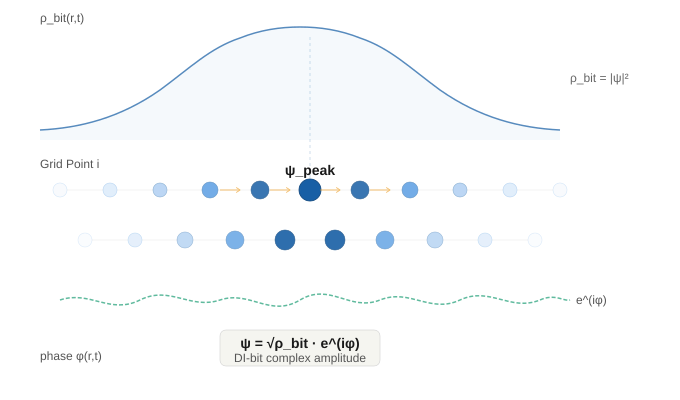
\includegraphics[width=0.90\textwidth]{qm2040a_fig1_gaussian_packet.pdf}
\caption{Gaussian Sea-polarization wave packet on the 600-cell lattice.
  Grid Points (circles) are coloured by the local count register
  $\rho_{\rm bit}$ (dark blue $=$ high, pale blue $=$ low),
  following the Gaussian envelope $\rho_{\rm bit}(r,0) \propto
  e^{-r^2/2\sigma^2}$ shown as the upper curve.
  Amber arrows indicate the direction of coherent DI-bit messenger flow.
  The lower dashed curve shows the phase oscillation $e^{i\phi}$ ---
  the rotation of each site's $\SSV_{\rm net}$ orientation.
  The site field $\psi = \sqrt{\rho_{\rm bit}}\,e^{i\phi}$
  encodes the count and orientation registers at each Grid Point.}
\label{fig:gaussian}
\end{figure}

%=====================================================================
\section{Lattice Hopping Hamiltonian}
%=====================================================================

Over one tick $\Delta t = \tP$ the amplitude at site $i$ evolves as
\begin{equation}
\psi_i(t+\Delta t) = \psi_i(t) - \frac{i\Delta t}{\hbar}
\sum_j H_{ij}\,\psi_j(t),
\label{eq:evolution}
\end{equation}
where
\begin{equation}
H_{ij} = \begin{cases}
-T & j \sim i \text{ (nearest neighbour)}, \\
+z\,T & j = i, \quad z = 12, \\
0 & \text{otherwise},
\end{cases}
\quad T = \frac{\hbar^2}{4m\,\Delta s^2}.
\label{eq:H}
\end{equation}

The factor $-i/\hbar$ is not postulated; it is grounded in the
geometry and dynamics of the phase register.

\begin{proposition}[Origin of unitarity and the imaginary unit;
derivation-sketch grade, conditional on FI-QMRG-1 and B-QMRG-1]
\label{prop:unitarity}
The per-Moment update of the site field is unitary, with
continuous-time generator of the form $-\tfrac{i}{\hbar}H$,
$H$ Hermitian.
\end{proposition}

\begin{proof}[Argument]
Three substrate facts combine.
(i)~\emph{Norm conservation:} $\sum_i \rho_i$ is the total count
register, conserved per Moment by the Nexus; hence
$\sum_i|\psi_i|^2$ is conserved.  Nothing about phase enters this
clause.
(ii)~\emph{Reversibility:} PCD displacement is deterministic and
invertible (A1--A9 rules; the substrate has no diffusive or
stochastic process), so the per-Moment map is invertible.
(iii)~\emph{Linearity:} $\SSV_{\rm net}$ is by definition the vector
sum of arriving contributions, and vector summation of planar
vectors with magnitudes $\sqrt{\rho_j}$ and angles $\phi_j$ \emph{is}
complex addition of the $\psi_j$; in the coherent weak-field regime
(B-QMRG-1) the per-Moment refresh therefore acts linearly on the
site fields, and superposition of patterns is vector addition of
their $\SSV_{\rm net}$ contributions.
An invertible, norm-preserving, linear update on a complex site
field is unitary; its continuous-time generator is
$-\tfrac{i}{\hbar}H$ with $H$ Hermitian, which is exactly the
tight-binding form~\eqref{eq:evolution}.  Under FI-QMRG-1 the
imaginary unit has a concrete substrate meaning: multiplication by
$-i$ is a quarter-turn of $\SSV_{\rm net}$ in the distinguished
plane --- the generator of pattern rotation.  Classical diffusion
would replace $-i$ by a real positive $D$; the substrate excludes
this because its update is reversible (clause~ii), whereas diffusion
is not.
\end{proof}

\begin{remark}[Grade and registered obligations (CONV-014)]
Proposition~\ref{prop:unitarity} is carried at derivation-sketch
grade (panel-ratified 4--1): clauses (i) and (ii) are corpus-level
substrate facts; clause (iii) consumes the bridging input B-QMRG-1
(coherent-mode amplitude--count relation) and the small-signal
linear-response regime.  Registered obligations \emph{(terminal statuses per the CONV-016
adjudication, Patch 3008: sector conditionality RESOLVED; the
remaining items are ORDINARY registered research, not conditions on
this paper's standing — OPEN-QMRG-ETA (COMPLETE as closure candidate: mode-independence
derived at 3009; the value $c_{\rm geo} = z = 12$ computed at 3010
for the standing class with verified physical inertness; batched for
the next panel touchpoint),
OPEN-QMRG-UNIQ, and watch condition W-MULTILINK-1; citation-note
requirements persist only for the E-2 note classes:
uniqueness, universal-microscopic claims --- the physical
$\rho$-calibrated-normalization note class was DISCHARGED at
bookkeeping grade (CONV-013 AUX-3, recorded Patch 3037), and the
$\eta$-universality note class was DISCHARGED at CONV-017 AUX-2
(5/5, riding AUX-1 CLOSE: the ALL-MODES lemma + coverage sweep;
recorded Patch 3050; grade fence per the 3038 labels — closed at
bookkeeping/derivation grade, not every microscopic realization))}. Interim statuses as of
the CONV-015 adjudication (Patch 3004), retained for the record: \textbf{OPEN-QMRG-B1 --- CLOSED at
proportionality grade (panel 5--0)}; the load-bearing derivation is
the dynamical energy balance (elastic quadratic storage + additive
messenger energy), with AP-2 serving as register identification
rather than premise, and the rival linear reading excluded
dynamically (it requires an arrival-phase discipline the substrate
lacks); the exact coefficient of the canonical normalization is addressed by
\textbf{OPEN-QMRG-B1-CONST --- DISPOSITION CANDIDATE, panel-pending
(Patch 3006)}: in the declared convention (cycle-averaged mean-square
in-plane register), the coefficient is \emph{derived} --- the
harmonic virial gives $\langle S_\perp^2\rangle = N\hbar/(\mu\omega)$
with coefficient exactly~1 given $E = N\hbar\omega$, and the
canonical per-quadrature $\tfrac12$ is the two-quadrature split of
the rotating ZBW pattern (a physical fact of rotation, not a
bookkeeping choice) --- while the one genuinely lattice-dependent
factor, the participation ratio $\eta \equiv \rho/N$, is formally
quarantined as a registered substrate parameter with a checkable
mode-independence claim; the derived layer is verified invariant
under turnover details (the separation is clean). Exact
$\rho$-calibrated amplitude claims, formerly barred pending
$\eta$'s lattice derivation, are DISCHARGED at bookkeeping grade
(v2.11; $\eta = c_{\rm geo} = 12$, standing class, inertness
measured --- Patches 3009/3010; panel discharge CONV-013 AUX-3;
class-scoped and grade-fenced per the Patch 3037 record: licensed
is $\rho = 12N$ substitution into convention-labeled identities,
nothing above bookkeeping grade). The QM-1$\leftrightarrow$QM-5
mutual-support prohibition is \textbf{DISCHARGED}: both papers cite
the independent derivation record, not each other, for the relation.
\textbf{R-4 --- CLOSED at derivation grade for the shipped
component-diagonal transport class (panel 5--0)}; the multi-edge-
correlated kernel question, spun off as
\textbf{OPEN-QMRG-R4-MULTILINK}, is now a \emph{resolution
candidate at registry-theorem grade, panel-pending (Patch 3005)}:
the committed refresh law forces the single-edge class by three
ratified clauses (A3$'$ additive vector-sum formation; AP-2 minimal
messenger content; A3$'$ per-Moment reset), the committed chirality
mechanism (per-edge scalar rate asymmetry, F.1) is component-diagonal
and hence plane-exact, and the excluded non-separable cross-product
class is verified to leak at order unity --- the exclusion, not a
bound, is the correct closure shape. Citations under
the widened bar carry the conditional note naming MULTILINK +
B1-CONST. Historical framing of the obligations as first registered:
\emph{OPEN-QMRG-B1 (original registration)}  The bridge $|\SSV_{{\rm net},\perp}|^2 \propto
\rho$ is derived from elastic energy balance: the eDP Sea's dipole
stiffness (the same $\kappa$ that sets $\mu_0,\epsilon_0$; SF-6
Tier~1/2) stores maintained energy quadratically; the A3$'$
per-Moment reset makes the register a driven steady state; each
messenger transfers the mode quantum $\hbar\omega$ ($E=\hbar\nu_C$).
Balance gives $|\SSV_{{\rm net},\perp}|^2 \propto N\hbar/(\mu\omega)$
--- the bridge WITH its constant, recovering the canonical
$1/(2\omega)$ per-quantum normalization as an \emph{output} (the
structure Paper~6 presupposes is predicted, not consumed: the
CONV-014 circularity concern is cut at its first link).  The
quadratic-vs-linear fork is decided by ratified AP-2: the rival
amplitude-like reading requires quadrature phase-locking and
contradicts the intensity-like clause (verified with negative
control; toy-model limits registered).  The mutual-support
prohibition remains formally in force pending adjudication, at which
it becomes dischargeable.
\textbf{R-4} --- plane stability: \emph{CLOSURE CANDIDATE at
derivation grade, panel-pending (Patch 3001).}  (i)~For the
component-diagonal transport this paper's update actually uses,
plane closure is \emph{exact at all orders}: a scalar stencil cannot
mix Cartesian components.  (ii)~For general direction-coupled
transport $T(v) = \alpha I + \beta v v^{\!\top}$, the
lattice-anisotropic out-of-plane channel is suppressed as
$(k\Delta s)^4$, because the twelve icosahedral neighbour directions
form a spherical \emph{5-design} (moments through order five exactly
isotropic; first anisotropy at order six) --- numerically verified
with an octahedron negative control, and bounded by
$(2\pi\lP/\lambda_C)^4 \approx 3\times10^{-90}$ per refresh.
(iii)~The remaining isotropic direction-coupled channel is
identified as the longitudinal/spin sector, not leakage error.
(iv)~Universality: under $E = \hbar\nu_C$ the rotation rate obeys
$\omega \ge mc^2/\hbar > 0$ on the full support, so the plane is
defined for stationary states as well.  Record:
\texttt{sketches/3001\_r4\_plane\_stability\_lemma.md};
verify \texttt{code/3001\_r4\_5design\_check.py} (ALL PASS).  The theorem of
\S4 consumes only the \emph{form} of the update (complex, linear,
Hermitian-generated), which this proposition supplies conditionally.
\end{remark}

\begin{remark}[Why $T = \hbar^2/(4m\Delta s^2)$, not $\hbar^2/(2m\Delta s^2)$]
The icosahedral 600-cell has $z=12$ nearest neighbours in 3D.
The graph Laplacian over all 12 neighbours yields
$(\mathcal{A}\psi)/\Delta s^2 \to 2\nabla^2\psi$ (Appendix~A).
The factor 2 is absorbed into the denominator of $T$: with
$T = \hbar^2/(4m\Delta s^2)$ and the factor of 2 from the Laplacian,
$-T \times 2\Delta s^2\nabla^2\psi = -\hbar^2\nabla^2\psi/(2m)$,
which is the correct kinetic operator.
Using $T = \hbar^2/(2m\Delta s^2)$ would give $-\hbar^2\nabla^2\psi/m$
(wrong by a factor of 2).
\end{remark}

%=====================================================================
\section{Continuum Limit: The Schr\"{o}dinger Equation}
%=====================================================================

\begin{theorem}[Schr\"{o}dinger equation from DI-bit hopping]
\label{thm:schrodinger}
In the continuum limit $\Delta s \to 0$ (holding $T\Delta s^2
= \hbar^2/(4m)$ fixed), the discrete hopping equation~\eqref{eq:evolution}
becomes
\begin{equation}
i\hbar\,\frac{\partial\psi}{\partial t}
= -\frac{\hbar^2}{2m}\nabla^2\psi + V(\mathbf{r})\psi,
\label{eq:Schrodinger}
\end{equation}
where $V(\mathbf{r}) = -k_{\rm PSR}\,\Delta|\SSV(\mathbf{r})|$ is
the external potential sourced by the Space Stress Vector field.
\end{theorem}

\begin{proof}
From the 600-cell graph Laplacian (Appendix~A):
$\sum_{j\sim i}(\psi_j - \psi_i) = 2\Delta s^2\nabla^2\psi
+ O(\Delta s^4)$.  Substituting into~\eqref{eq:evolution}:
\begin{equation}
i\hbar\,\frac{\psi_i(t+\Delta t) - \psi_i(t)}{\Delta t}
= -T\bigl(\mathcal{A}\psi\bigr)_i + V_i\psi_i
= -\frac{\hbar^2}{4m\Delta s^2}\cdot 2\Delta s^2\nabla^2\psi + V\psi
= -\frac{\hbar^2}{2m}\nabla^2\psi + V\psi.
\end{equation}
Taking $\Delta t \to 0$ gives~\eqref{eq:Schrodinger}. \qed
\end{proof}

\begin{remark}[Origin of the potential term]
The potential enters the phase evolution as the first-order
modulation of the pattern rotation rate,
$\omega_{\rm local} = (mc^2 + V_{\SSV})/\hbar$
(\S2, under the corpus identification $E = \hbar\nu_C$): a region of
higher $\SSV$ shifts the local relation between pattern rotation and
coordinate time --- the same $\SSV\!\to$ tick machinery that produces
time dilation in the relativity sector.  The diagonal term
$V_i\psi_i$ in the discrete update is this modulation written
site-wise.
\end{remark}

\begin{figure}[H]
\centering
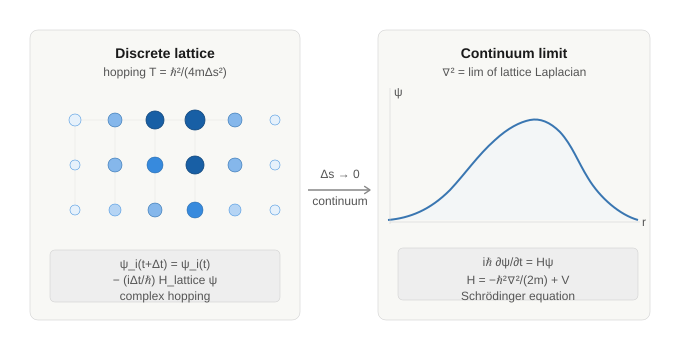
\includegraphics[width=0.90\textwidth]{qm2040a_fig2_discrete_continuum.pdf}
\caption{Discrete-to-continuum transition.
  \textit{Left:} Discrete 600-cell lattice with DI-bit amplitudes
  (colour $=$ density, arrows $=$ hopping direction).  The master equation
  governs complex amplitude hopping at each tick.
  \textit{Right:} Smooth wavefunction $|\psi(r,t)|^2$ from the continuum
  limit.  The lattice Laplacian $(\mathcal{A}\psi)/\Delta s^2 \to 2\nabla^2\psi$
  connects the two descriptions via Theorem~\ref{thm:schrodinger}.}
\label{fig:discrete_continuum}
\end{figure}

%=====================================================================
\section{Madelung Decomposition and Quantum Pressure}
%=====================================================================

\begin{proposition}[Madelung transformation]
Writing $\psi = \sqrt{\rho}\,e^{iS/\hbar}$ and substituting
into~\eqref{eq:Schrodinger} gives the real pair:
\begin{align}
\frac{\partial\rho}{\partial t}
+ \nabla\cdot\!\left(\rho\,\frac{\nabla S}{m}\right) &= 0,
\label{eq:continuity}\\
\frac{\partial S}{\partial t}
+ \frac{(\nabla S)^2}{2m} + V - Q &= 0,
\label{eq:HJ}
\end{align}
where the quantum pressure is
$Q = -\hbar^2\nabla^2\!\sqrt{\rho}/(2m\sqrt{\rho})$.
\end{proposition}

Equation~\eqref{eq:continuity} is DI-bit number conservation, enforced
by the Nexus.  The quantum pressure $Q$ in~\eqref{eq:HJ} is the
geometric interference effect of Sea-polarization pattern
contributions arriving from regions of different density --- planar
$\SSV_{\rm net}$ vectors summing with different orientations; it is
not postulated but emerges automatically from the complex hopping.

%=====================================================================
\section{Predictions}
%=====================================================================

At all laboratory wavelengths $\lambda \gg \lP$, lattice corrections
to quantum dynamics are of order $(\lP/\lambda)^2 \lesssim 10^{-58}$
(optical) and unobservable.  In the energy spectrum of bound states:
\begin{equation}
E_n^{\rm CPP} = E_n^{\rm QM}\bigl[1 + c_n(\lP/\lambda_n)^2
+ O(\lP/\lambda_n)^4\bigr].
\end{equation}
These corrections are in principle falsifiable: a measurement of
atomic energy levels at precision $\gg 10^{-50}$ relative accuracy
would probe the lattice structure.

%=====================================================================
\section{Conclusion}
%=====================================================================

The Schr\"{o}dinger equation emerges in CPP from the per-Moment
dynamics of the Sea-polarization pattern on the 600-cell lattice.
The site field reads the two registers the Grid-Point state protocol
already holds: the count ($\rho \leftrightarrow \SSV_{\rm abs}$) and
the orientation ($\phi \leftrightarrow \SSV_{\rm net}$ direction in
the ZBW plane) --- the grounding adds no state to the substrate.
DI-bits are stateless couriers; the phase belongs to the pattern
they refresh, rotating at the Compton rate $\omega_C = mc^2/\hbar$.
The derivation uses no diffusion step; the imaginary unit is the
quarter-turn generator of pattern rotation, and unitarity follows
from reversible, count-conserving PCD dynamics
(Proposition~\ref{prop:unitarity}, derivation-sketch grade with
named inputs FI-QMRG-1 and B-QMRG-1).  The quantum pressure term is
automatic, not postulated.  The key numerical results are unchanged
from v1.x: $T = \hbar^2/(4m\Delta s^2)$, not
$\hbar^2/(2m\Delta s^2)$, to account for the factor of 2 from the
12-neighbour graph Laplacian of the 600-cell; and the phase-advance
rate $mc\Delta s/\hbar$, now correctly attributed to the pattern's
ZBW rotation rather than to courier-carried accumulation.

%=====================================================================
\appendix
\section{Graph Laplacian of the 600-Cell in 3D}
\label{app:laplacian}
%=====================================================================

The 600-cell has coordination number $z=12$ in 3D ($d=3$).
For a smooth function $\psi(\mathbf{r})$ and vertex $i$ at $\mathbf{r}_i$:
\begin{equation}
\sum_{j\sim i}(\psi_j - \psi_i)
= \tfrac{1}{2}\,\frac{z\,\Delta s^2}{d}\,\nabla^2\psi + O(\Delta s^4)
= 2\,\Delta s^2\,\nabla^2\psi + O(\Delta s^4).
\end{equation}
The first step uses icosahedral symmetry ($\sum_j\Delta\mathbf{r}_{ij}=0$,
$\sum_j(\Delta\mathbf{r}_{ij})^2 = z\Delta s^2\mathbf{1}/d$);
the numerical value $z/(2d) = 12/6 = 2$ is a property of the 600-cell.

%=====================================================================

\section*{Acknowledgements}
The CPP programme is registered at OSF (DOI:~\url{https://doi.org/10.17605/OSF.IO/JXE8D}) and maintained at GitHub (\url{https://github.com/Hyperphysics-Institute/CPP}).

\bibliographystyle{plainnat}
\bibliography{cpp_qm_series}

\end{document}
